<<<<<<< HEAD
\documentclass[titlepage]{article}
\author{Ryan Kwon, Anthoney Tsou}
\title{An Implementation of Quality Minus Junk}
\usepackage{Sweave}
\begin{document}
\Sconcordance{concordance:paper.tex:paper.Rnw:%
1 2 1 1 0 6 1 5 0 1 4 10 1 1 2 1 0 1 1 1 2 1 0 1 2 1 0 1 2 5 0 1 5 2 0 %
3 1 3 0 1 2 3 1 4 0 1 3 3 1 4 0 1 3 2 1 1 2 1 0 2 1 24 0 1 4 5 0 1 3 8 %
0 1 2 1 3 2 0 1 1 3 0 1 3 8 0 1 2 1 4 3 0 1 2 1 0 1 2 25 0 1 2 2 1 1 3 %
2 0 1 1 18 0 1 5 3 0 1 1 18 0 1 4 2 0 1 1 18 0 1 6 4 0 1 1 19 0 1 2 5 1 %
5 0 1 4 5 0 1 4 5 0 1 4 6 1 7 0 1 6 5 0 1 4 46 1}

\maketitle
=======
\documentclass[12pt]{article}
\usepackage{listings}
\usepackage{Sweave}
\begin{document}
\Sconcordance{concordance:paper.tex:paper.Rnw:%
1 2 1 1 0 6 1 5 0 1 4 10 1 1 2 1 0 1 1 1 2 1 0 1 2 1 0 1 2 5 0 1 5 2 0 %
3 1 3 0 1 2 3 1 4 0 1 3 3 1 4 0 1 3 2 1 1 2 1 0 2 1 24 0 1 4 5 0 1 3 8 %
0 1 2 1 3 2 0 1 1 3 0 1 3 8 0 1 2 1 4 3 0 1 2 1 0 1 2 25 0 1 2 2 1 1 3 %
2 0 1 1 18 0 1 5 3 0 1 1 18 0 1 4 2 0 1 1 18 0 1 6 4 0 1 1 19 0 1 2 5 1 %
5 0 1 4 5 0 1 4 5 0 1 4 6 1 7 0 1 6 5 0 1 4 46 1}


\section*{Installation}
To install the package:

\begin{Schunk}
\begin{Sinput}
> #library(devtools)
> #install_github("rynkwn/qmj")
\end{Sinput}
\end{Schunk}
>>>>>>> eb2579c12852abb8686cb1a74a3155acd63994cb

\section*{Background}
qmj implements the results and methodology of the paper \emph{Quality Minus Junk} by Clifford Asness, Andrea Frazzini, Lasse Pedersen. In their paper, they use several measures to calculate the relative profitability, growth, safety, and payouts of a company, which they use to provide an overall quality score for a company.

This quality score is used to recommend which companies to buy and which to sell, by reasoning that quality companies are likely to outperform the market, while ``junk'' companies are likely to underperform relative to the market.

Here we use the equations and methods described in the paper, coupled with data taken from reputable online sources, in order to produce quality measurements for companies listed in the Russell 3000 Index.

\section*{Getting Started}
In order to start you off, qmj comes equipped with several data sets, including company information, financial statements, and daily stock data. To access them, call:

\begin{Schunk}
\begin{Sinput}
> library(qmj)
> data(companies) #Stores company names and tickers from the 
> #Russell 3000 index
> data(financials) #Stores financial documents for the given 
> #list of companies.
> data(prices) # Stores price returns and closing stock prices 
> #for the past two years.
> data(quality) #Stores the quality scores and the scores of 
> #its components.
\end{Sinput}
\end{Schunk}
\begin{Schunk}
\begin{Sinput}
> #And more detailed data sets into what makes up quality
> data(profitability)
> data(growth)
> data(payouts)
> data(safety)
\end{Sinput}
\end{Schunk}

Getting a quality data frame and a holistic summary of all its components can be done by calling

\begin{Schunk}
\begin{Sinput}
> #market_data(companies, financials, prices)
\end{Sinput}
\end{Schunk}

If you're only interested in accessing certain quality factors, such as profitability, as well as what makes it up (such as gross profits over assets (GPOA), or cash flow over assets (CFOA)) call

\begin{Schunk}
\begin{Sinput}
> #market_profitability(companies, financials)
\end{Sinput}
\end{Schunk}

\section*{Analyzing your Data}
The qmj package has stored a large number of qmj objects, which store significant amounts of information about a single company and which allows more in-depth analysis of that company. Some examples of analysis follow:
\begin{Schunk}
\begin{Sinput}
> data(qmjs)
> first_qmj <- qmjs[[1]]
> summarize(first_qmj) # Displays key information about this qmj object.
\end{Sinput}
\begin{Soutput}
Information for:  FLWS
_______________________________________
Quality Score:  0.3588747
_______________________________________
  profitability     GPOA         ROE       ROA      CFOA      GMAR       ACC
1     0.2911018 0.262272 -0.01867136 0.2019969 0.1198031 0.2308763 0.1606091


       growth        GPOA ROE        ROA        CFOA        GMAR        ACC
1 -0.03357491 -0.03355643   0 0.02050147 -0.01102495 -0.05582183 0.01561731


       safety      BAB       IVOL          LEV OhlsonOScore AltmanZScore
1 -0.08842572 0.142523 -0.2184943 -0.009880442            0            0


    payouts      EISS       DISS       NPOP
1 0.1897736 0.1998357 0.09870005 0.01514234

_______________________________________
\end{Soutput}
\begin{Sinput}
> #We're clearly missing some interesting data, but we can still 
> #perform some analysis.
> data(safety)
\end{Sinput}
\end{Schunk}
\begin{Schunk}
\begin{Sinput}
> plot_safety(first_qmj, safety)
\end{Sinput}
\begin{Soutput}
[1] "Selected object is in the yellow bin."
\end{Soutput}
\end{Schunk}
<<<<<<< HEAD
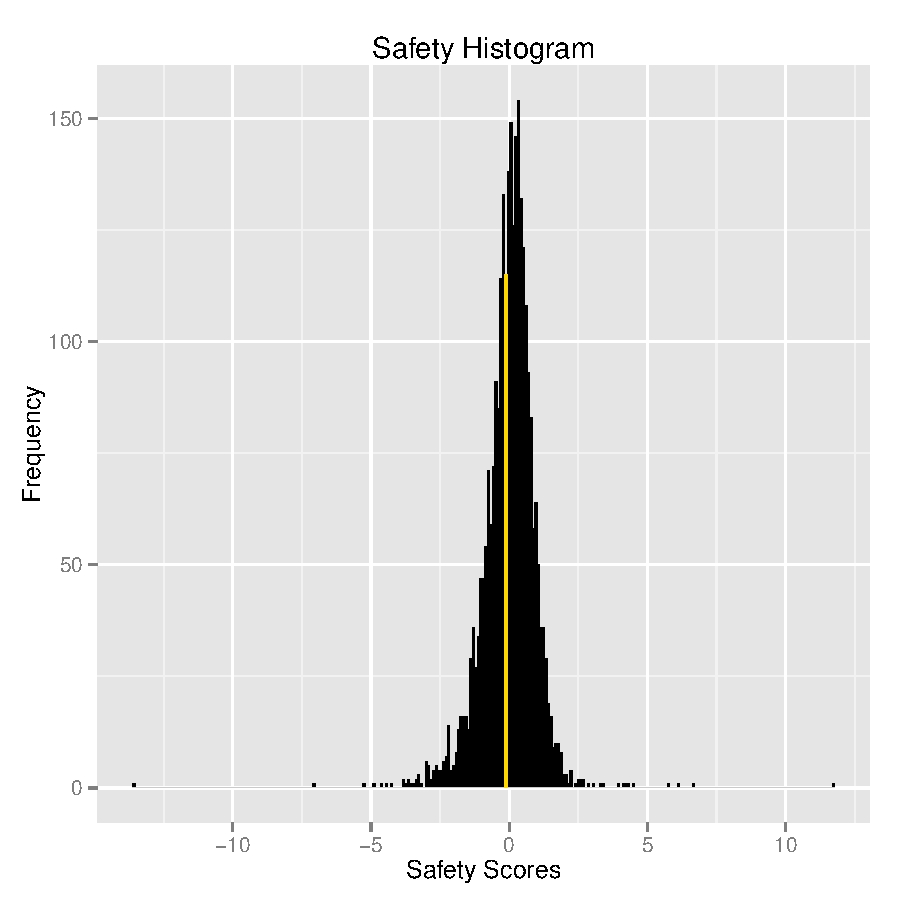
\includegraphics{paper-006}
=======
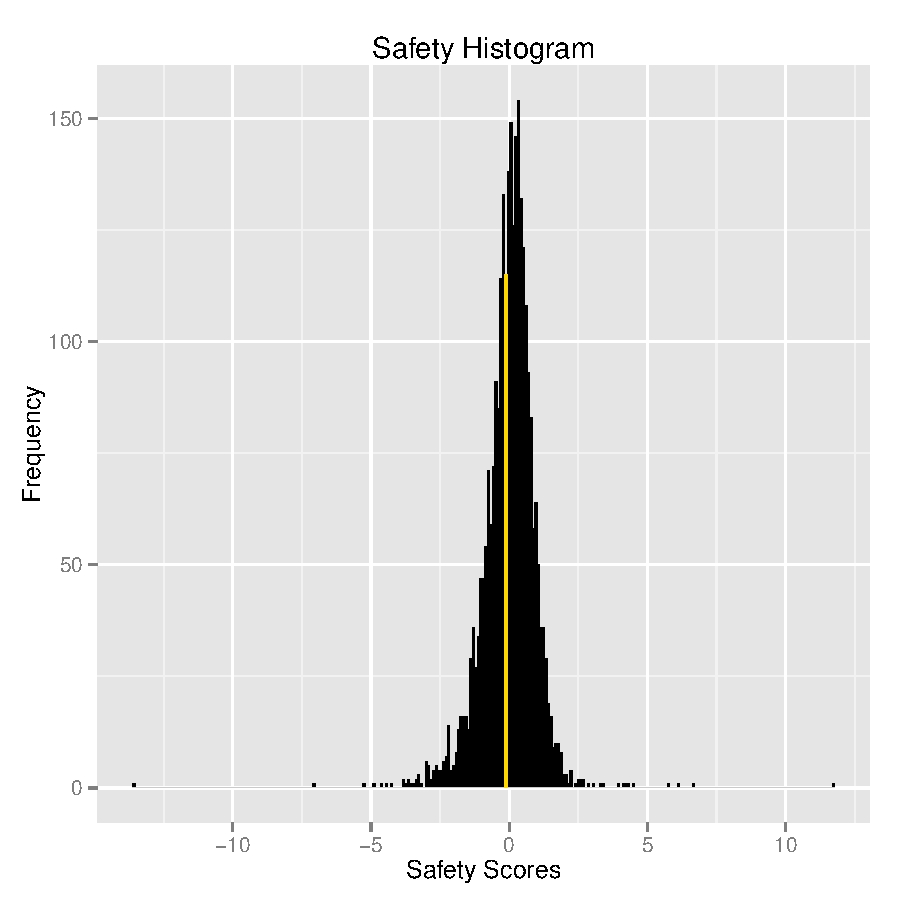
\includegraphics{paper-007}
>>>>>>> eb2579c12852abb8686cb1a74a3155acd63994cb

\begin{Schunk}
\begin{Sinput}
> #Now let's look at a graph for quality.
> data(quality)
> second_qmj <- qmjs[[2]]
\end{Sinput}
\end{Schunk}
\begin{Schunk}
\begin{Sinput}
> plot_quality(second_qmj, quality)
\end{Sinput}
\begin{Soutput}
[1] "Selected object is in the yellow bin."
\end{Soutput}
\end{Schunk}
<<<<<<< HEAD
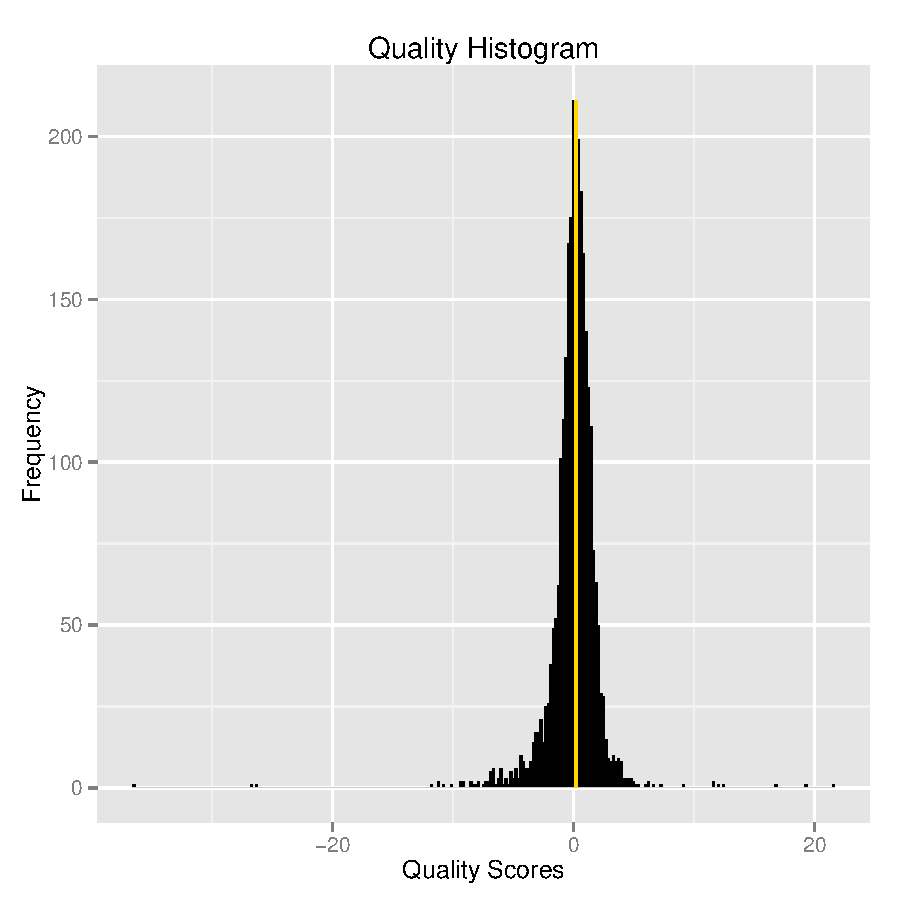
\includegraphics{paper-008}
=======
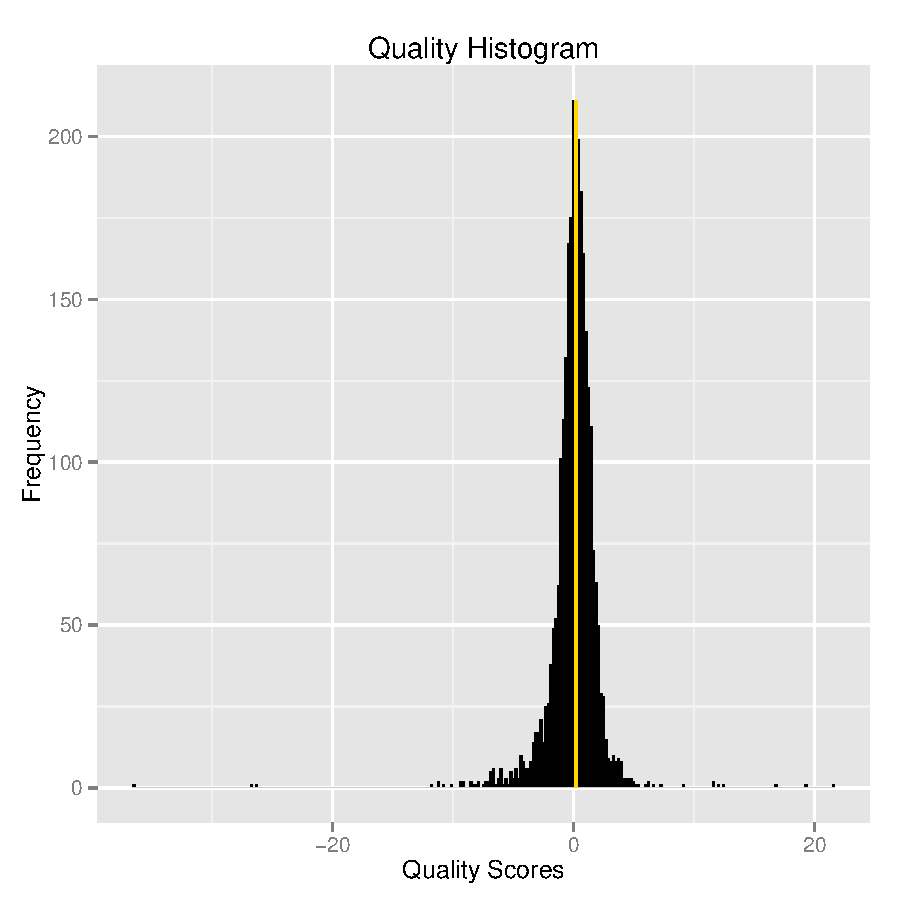
\includegraphics{paper-009}
>>>>>>> eb2579c12852abb8686cb1a74a3155acd63994cb

\begin{Schunk}
\begin{Sinput}
> #What if I'm only interested in looking closely at a few companies? 
> #Well, voila.
> desired_companies <- c("GOOG", "IBM", "FLWS")
> #Returns a list containing the given qmj objects in order.
> desired_qmjs <- get_qmjs(desired_companies, qmjs) 
> summarize(desired_qmjs[[1]])
\end{Sinput}
\begin{Soutput}
Information for:  GOOG
_______________________________________
Quality Score:  0.4324132
_______________________________________
  profitability     GPOA        ROE        ROA       CFOA      GMAR        ACC
1     0.1768459 2.118874 -0.2618723 -0.8683505 -0.5174924 0.4885829 -0.3784276


       growth        GPOA ROE        ROA        CFOA        GMAR        ACC
1 -0.03648541 -0.02796106   0 0.01365657 -0.01396494 -0.05372761 0.01214001


      safety        BAB      IVOL       LEV OhlsonOScore AltmanZScore
1 -0.2362488 -0.3126085 0.7353582 0.3042633   -0.6317125   -0.6706373


    payouts      EISS      DISS      NPOP
1 0.5283014 0.1308389 0.7281532 0.0142409

_______________________________________
\end{Soutput}
\end{Schunk}

But the package also provides some tools for better examining your data en masse, as opposed to individual companies.

\begin{Schunk}
\begin{Sinput}
> #Let's look at the head of our quality data frame.
> data(quality)
> head(quality)
\end{Sinput}
\begin{Soutput}
                     name ticker profitability      growth      safety
1         ANGIES LIST INC   ANGI    -0.1575365 24.55764246 -0.89076389
2 SEACOAST BANKING CORP F   SBCF    -0.9552288 21.17749195  0.23623565
3                  AMERCO   UHAL    -0.3350943 19.25596295 -0.16064717
4   GUIDANCE SOFTWARE INC   GUID     0.2245725 13.61798234  0.09569998
5       BROWN & BROWN INC    BRO     0.1484205 -0.04063592 11.76587071
6 CAPITOL FEDERAL FINL IN   CFFN     5.7540587 -0.04904148  5.73770806
     payouts  quality
1 -1.8699982 21.63934
2 -1.0820805 19.37642
3 -1.9855567 16.77466
4 -1.5591484 12.37911
5  0.2254432 12.09910
6  0.2292110 11.67194
\end{Soutput}
\begin{Sinput}
> #Angies has an abnormally high growth score, which is very suspicious.
> #Companies that are primarily driven by a single component score 
> #are suspect, so let's filter out companies that are driven by growth.
> sans_growth <- filter_companies(quality, filter="growth")
> head(sans_growth)
\end{Sinput}
\begin{Soutput}
                      name ticker profitability      growth     safety
5        BROWN & BROWN INC    BRO     0.1484205 -0.04063592 11.7658707
6  CAPITOL FEDERAL FINL IN   CFFN     5.7540587 -0.04904148  5.7377081
8      CENTURY ALUMINUM CO   CENX    -0.1912805  3.43982232  6.1767505
9  CORRECTIONS CORP OF AME    CXW    -0.3283571  3.22020489  4.1009744
10    ROUSE PROPERTIES INC    RSE     3.6209141  0.04701919  1.8876675
11       PATTERSON COS INC   PDCO    -0.7411908 -0.05296278  0.1659304
      payouts   quality
5   0.2254432 12.099098
6   0.2292110 11.671936
8  -0.1956603  9.229632
9   0.1910389  7.183861
10  0.9855644  6.541165
11  6.7805708  6.152348
\end{Soutput}
\begin{Sinput}
> #On the other hand, if we're interested in only companies that are 
> #driven by growth, we can do the following:
> driven_by_growth <- filter_companies(quality, filter="growth", remove=FALSE, isolate=TRUE)
> head(driven_by_growth)
\end{Sinput}
\begin{Soutput}
                      name ticker profitability   growth      safety    payouts
1          ANGIES LIST INC   ANGI   -0.15753650 24.55764 -0.89076389 -1.8699982
2  SEACOAST BANKING CORP F   SBCF   -0.95522880 21.17749  0.23623565 -1.0820805
3                   AMERCO   UHAL   -0.33509433 19.25596 -0.16064717 -1.9855567
4    GUIDANCE SOFTWARE INC   GUID    0.22457246 13.61798  0.09569998 -1.5591484
7       UTAH MED PRODS INC   UTMD   -3.30709253 16.48412 -1.72466975  0.1363612
38       NEWBRIDGE BANCORP   NBBC   -0.05392051  3.83622 -0.17048483  0.2178660
    quality
1  21.63934
2  19.37642
3  16.77466
4  12.37911
7  11.58872
38  3.82968
\end{Soutput}
\begin{Sinput}
> #We can also remove all companies with quality scores which are 
> #primarily driven by any component.
> #Notice that the remove parameter is by default TRUE, and 
> #isolate is by default FALSE
> liberal_arts_companies <- filter_companies(quality, filter="all")
> head(liberal_arts_companies)
\end{Sinput}
\begin{Soutput}
                      name ticker profitability      growth    safety   payouts
6  CAPITOL FEDERAL FINL IN   CFFN     5.7540587 -0.04904148 5.7377081 0.2292110
21 HANNON ARMSTRONG SUSTAI   HASI     1.2166640 -0.02772366 1.7356800 1.7275803
22  ADAMAS PHARMACEUTICALS   ADMS     1.6916207  0.50007697 2.2264045 0.2107355
24   OPLINK COMMUNICATIONS   OPLK     0.9992939  1.89816751 1.2105671 0.2178525
33              WATSCO INC    WSO     1.9397013 -0.01815565 1.8758314 0.1712876
34          P C CONNECTION   PCCC     1.4991871 -0.01996304 0.5011669 1.9790272
     quality
6  11.671936
21  4.652201
22  4.628838
24  4.325881
33  3.968665
34  3.959418
\end{Soutput}
\end{Schunk}


\section*{Updating your Data}
If you're interested in inputting your own data, you can generate financial statements for a data frame of companies as follows:

\begin{Schunk}
\begin{Sinput}
> #companies #Your custom data frame of company names and tickers. 
> #The column name for tickers must be "ticker"
\end{Sinput}
\end{Schunk}
\begin{Schunk}
\begin{Sinput}
> #rawdata <- get_info(companies) #Retrieves raw financial 
> #statements from google finance through the quantmod package.
\end{Sinput}
\end{Schunk}
\begin{Schunk}
\begin{Sinput}
> #financials <- tidyinfo(rawdata) #Renders raw data in a format 
> #usable by other functions in this package.
\end{Sinput}
\end{Schunk}

get\_info temporarily saves your progress to the extdata folder at all stages of its process, allowing you to resume your downloading if the process is interrupted for any reason.

\subsection*{Updating Prices}
Updating prices is a separate, lengthy process, and for that reason is separated from the other functions that automatically collect financial statements. To update prices, which is necessary for calculating safety measurements, call:

\begin{Schunk}
\begin{Sinput}
> # rawprices <- get_prices(companies) #Retrieves stock price 
> #data from Google Finance for listed companies for the past 
> #two years. Also saves data from the S&P 500, retrieved from 
> #Yahoo Finance.
\end{Sinput}
\end{Schunk}
\begin{Schunk}
\begin{Sinput}
> # prices <- tidy_prices(rawprices) #Renders the raw data into 
> #a form usable by other functions in this package.
\end{Sinput}
\end{Schunk}

The get\_prices function is able to save its progress as it temporarily saves its download data to the extdata folder in the package's folder.
<<<<<<< HEAD
=======

\section*{Conclusion}

In the \textbf{qmj} package, we automate AQR's method of assigning quality scores for publicly traded companies in today's market. The package itself provides convenient datasets and utility functions, and it also takes advantage of R's robust nature to allow seamless interaction with functions in the base R package and other packages.
\\
\\
\emph{Ryan Kwon}
\\
\emph{Williams College}
\\
\emph{Williamstown, MA}
\\
\emph{USA}
\\
rhk1@williams.edu
\\
\\
\emph{Anthoney Tsou}
\\
\emph{Williams College}
\\
\emph{Williamstown, MA}
\\
\emph{USA}
\\
at6@williams.edu

\section*{Bibliography}
Asness, Clifford S., Andrea Frazzini, and Lasse H. Pedersen. ``Quality Minus Junk." AQR (2014)
\section*{Appendix}
We calculate quality scores for publicly traded companies in the Russell 3000 Index by summing the z-scores for each company's profitability, growth, safety, and payouts. We attempt to perform the same calculations as AQR does, but we have a few adjustments given the availability of data from public sources. 
\subsection*{Profitability}
Profitability is composed of six variables: gross profits over assets ($GPOA$), return on equity ($ROE$), return on assets ($ROA$), cash flow over assets ($CFOA$), gross margin ($GMAR$), and accruals ($ACC$). $GPOA$ is calculated as gross profits ($GPROF$) over total assets ($TA$). $$GPOA \ = \ \frac{GPROF}{TA}$$ $ROE$ is calculated as net income ($NI$) over book equity ($BE$), which is shareholders' equity (the difference of Total Liabilities and Shareholders' Equity ($TLSE$) with Total Liabilities ($TL$)) - preferred stock (the sum of redeemable preferred stock ($RPS$) and non redeemable preferred stock ($NRPS$)). $$ROE \ = \ \frac{NI}{BE}$$ $ROA$ is calculated as $NI$ over $TA$. $$ROA \ = \ \frac{NI}{TA}$$ $CFOA$ is calculated as $NI$ + depreciation ($DP.DPL$) - changes in working capital ($CWC$) - capital expenditures ($CX$) all over $TA$. $$CFOA \ = \ \frac{NI \ + \ DP.DPL \ - \ CWC \ - \ CX}{TA}$$ $GMAR$ is calculated as $GPROF$ over total revenue ($TREV$). $$GMAR \ = \ \frac{GPROF}{TREV}$$ Finally, $ACC$ is calculated as $DP.DPL$ - $CWC$ all over $TA$. $$ACC \ = \ \frac{DP.DPL \ - \ CWC}{TA}$$ We then standardize all components of profitability to z-scores and then standardize all profitability scores into z-scores. $$Profitability \ = \ z(z_{gpoa} \ + \ z_{roe} \ + \ z_{roa} \ + \ z_{cfoa} \ + \ z_{gmar} \ + \ z_{acc})$$
\subsection*{Growth}
Growth is measured by differences in profitability across a time span of four years. Though AQR recommends measuring growth across a time span of five years, public information that is both consistent and well-organized in 10-K forms is only available for a time span of four years, and it is still too early in the most recent year (2015) for most companies to have submitted a 10-K form. Thus, we measure growth using a time span of four years, which we will update once this year's 10-K form is submitted for each company in the Russell 3000 Index. As of now, $$Growth \ = \ z(z_{\Delta gpoa_{t,t-4}} \ + \ z_{\Delta roe_{t,t-4}} \ + \ z_{\Delta roa_{t,t-4}} \ + \ z_{\Delta cfoa_{t,t-4}} \ + \ z_{\Delta gmar_{t,t-4}} \ + \ z_{\Delta acc_{t,t-4}})$$
\subsection*{Safety}
Safety is composed of six variables: beta ($BAB$), idiosyncratic volatility ($IVOL$), leverage ($LEV$), Ohlson's O ($O$), Altman's Z ($Z$), and earnings volatility ($EVOL$). $BAB$ is calculated as the negative covariance of each company's daily price returns ($pret_{c_i}$) relative to the benchmark daily market price returns ($pret_{mkt}$), in this case the S\&P 500, over the variance of $pret_{mkt}$. $$BAB \ = \ \frac{-cov(pret_{c_i},pret_{mkt})}{var(pret_{mkt})}$$ $IVOL$ is the standard deviation of daily beta-adjusted excess returns. In other words, $IVOL$ is found by running a regression on each company's price returns and the benchmark, then taking the standard deviation of the residuals. Leverage is -(total debt ($TD$) over $TA$). $$Leverage \ = \ -\frac{TD}{TA}$$ 
\\
$$ O \ = \ -(-1.32 \ - \ 0.407 \ * \ log\left(\frac{ADJASSET}{CPI}\right) \ + \ 6.03 \ * \ TLTA \ - \ 1.43 \ * \ WCTA$$
$$ + \ 0.076 \ * \ CLCA \ - \ 1.72 \ * \ OENEG \ - \ 2.37 \ * \ NITA \ - \ 1.83 \ * \ FUTL$$
$$ + \ 0.285 \ * \ INTWO \ - \ 0.521 \ * \ CHIN)$$ 
$ADJASSET$ is adjusted total assets, which is $TA$ + 0.1 * (market equity ($ME$, calculated as average price per share for the most recent year * total number of shares outstanding ($TCSO$) - $BE$)). $$ADJASSET \ = \ TA \ + \ 0.1 \ * \ (ME \ - \ BE)$$ $CPI$, the consumer price index, is assumed to be 100, since we only care about the most recent year. $TLTA$ is book value of debt ($BD$, calculated as $TD$ - minority interest ($MI$) - ($RPS$ + $NRPS$)) over $ADJASSET$. $$TLTA \ = \ \frac{BD}{ADJASSET}$$ $WCTA$ is current assets ($TCA$) - current liabilities ($TCL$) over $TA$. $$WCTA \ = \ \frac{TCA - TCL}{TA}$$ $CLCA$ is $TCL$ over $TCA$. $$ CLCA \ = \ \frac{TCL}{TCA}$$ $OENEG$ is a dummy variable that is 1 if total liabilities ($TL$) is greater than $TA$. $$ OENEG \ = \ TL > TA $$ $NITA$ is $NI$ over $TA$. $$NITA \ = \ \frac{NI}{TA}$$ $FUTL$ is income before taxes ($IBT$) over $TL$. $$FUTL \ = \ \frac{IBT}{TL}$$ $INTWO$ is another dummy variable that is 1 if $NI$ for the current year and $NI$ for the previous year are both negative. $$INTWO \ = \ MAX(NI_t,NI_{t-1}) < 0$$ $CHIN$ is $NI$ for the current year - $NI$ for the previous year all over the sum of the absolute value of $NI$ for the current year and the absolute value of $NI$ for the previous year $$CHIN \ = \ \frac{NI_t \ - \ NI_{t-1}}{|NI_t| + |NI_{t-1}|}$$ Altman's Z is calculated using weighted averages of working capital ($WC$, calculated as $TCA$ - $TCL$), $$WC \ = \ TCA \ - \ TCL$$ retained earnings ($RE$, calculated as $NI$ - dividends per share ($DIVC$) * $TCSO$), $$RE \ = \ NI \ - \ DIVC \ * \ TCSO$$ earnings before interest and taxes ($EBIT$, calculated as $NI$ - Discontinued Operations($DO$) + ($IBT$ - income after tax ($IAT$)) + interest expense ($NINT$)), $$ EBIT \ = \ NI \ - \ DO \ + \ (IBT \ - \ IAT) \ + \ NINT $$ $ME$, and $TREV$, all over $TA$. $$Z \ = \frac{\ 1.2 \ * \ WC \ + \ 1.4 \ * \ RE \ + \ 3.3 \ * \ EBIT \ + \ 0.6 \ * \ ME \ + TREV}{TA}$$ $EBIT$ is likely an overestimate for a given company due to potentially missing information. $EVOL$ is calculated as the standard deviation of $ROE$ for a four year span. AQR recommends the past five years, but for the same reason stated in the Growth section, we use a four year span. $$EVOL = \sigma\left(\sum_{i=t-4}^{t}ROE_i\right)$$ Likewise, we standardize each variable and then standardize each safety measure, so $$Safety \ = \ z(z_{bab} \ + \ z_{ivol} \ + \ z_{lev} \ + \ z_{o} \ + \ z_{z} \ + \ z_{evol})$$ 
\subsection*{Payouts}
Payouts is composed of three variables: net equity issuance ($EISS$), net debt issuance ($DISS$), and total net payout over profits ($NPOP$). $EISS$ is calculated as the negative log of the ratio of $TCSO$ of the most recent year and $TCSO$ of the previous year. $$EISS \ = \ -log\left(\frac{TCSO_t}{TCSO_{t-1}}\right)$$ Though AQR uses split-adjusted number of shares, we are currently using $TCSO$ given available information and will adjust for splits in future iterations of qmj. $DISS$ is calculated as the negative log of the ratio of $TD$ of the most recent year and $TD$ of the previous year. $$DISS \ = \ -log\left(\frac{TD_t}{TD_{t-1}}\right)$$ $NPOP$ is calculated as $NI$ - $\Delta BE$ over a four year span all over sum of $GPROF$ for the past four years (for the same reason as explained in the Growth section). $$NPOP \ = \ \frac{NI - \Delta BE}{\sum_{i=t-4}^{t}GPROF_i}$$
>>>>>>> eb2579c12852abb8686cb1a74a3155acd63994cb
\end{document}
